\documentclass[format=sigchi, review=false, screen=true]{acmart}

\usepackage{booktabs} % For formal tables

% Metadata Information
%\acmJournal{FAT*}
\acmVolume{}
\acmNumber{}
\acmArticle{}
\acmYear{2019}
\acmMonth{9}
\copyrightyear{2019}
%\acmArticleSeq{9}
\acmConference[Preprint in Review]{ArXiV Computing Research Repository}{}

% DOI
\acmDOI{}

% Paper history
\received{April 2019}
\received[revised]{July 2019}
\received[revised]{August 2019}
%\received[accepted]{June 2009}


% Copyright
%\setcopyright{acmcopyright}
\setcopyright{acmlicensed}
%\setcopyright{rightsretained}
%\setcopyright{usgov}
%\setcopyright{usgovmixed}
%\setcopyright{cagov}
%\setcopyright{cagovmixed}

\usepackage[ruled]{algorithm2e} % For algorithms
\renewcommand{\algorithmcfname}{ALGORITHM}
\SetAlFnt{\small}
\SetAlCapFnt{\small}
\SetAlCapNameFnt{\small}
\SetAlCapHSkip{0pt}
\IncMargin{-\parindent}
% Arabic page numbers for submission.  Remove this line to eliminate
% page numbers for the camera ready copy
% \pagenumbering{arabic}

% Load basic packages
\usepackage{balance}       % to better equalize the last page
\usepackage{graphics}      % for EPS, load graphicx instead
\usepackage{todonotes}     % for \todo
%\usepackage[T1]{fontenc}   % for umlauts and other diaeresis
%\usepackage{txfonts}
%\usepackage{mathptmx}
%\usepackage[pdflang={en-US},pdftex]{hyperref}
%\usepackage{color}
\usepackage{booktabs}
\usepackage{subcaption}
\usepackage{textcomp}
\PassOptionsToPackage{warn}{textcomp}
%\usepackage[table]{xcolor}

% Some optional stuff you might like/need.
\usepackage{microtype}        % Improved Tracking and Kerning
% \usepackage[all]{hypcap}    % Fixes bug in hyperref caption linking
% \usepackage{ccicons}          % Cite your images correctly!
% \usepackage[utf8]{inputenc} % for a UTF8 editor only

% If you want to use todo notes, marginpars etc. during creation of
% your draft document, you have to enable the "chi_draft" option for
% the document class. To do this, change the very first line to:
% "\documentclass[chi_draft]{sigchi}". You can then place todo notes
% by using the "\todo{...}"  command. Make sure to disable the draft
% option again before submitting your final document.
%\usepackage{todonotes}

% Paper metadata (use plain text, for PDF inclusion and later
% re-using, if desired).  Use \emtpyauthor when submitting for review
% so you remain anonymous.


\newcommand{\FIXME}[1]{[\textbf{FIXME}: \textit{#1}]}

\newcommand\leadin[1]{%
    \vskip 5pt \noindent\textbf{#1.} %
}
\newcommand\leadinx[1]{%
    \vskip 5pt \noindent\textbf{#1} %
}

%
%\def\sharedaffiliation{%
%\end{tabular}
%\begin{tabular}{c}}
%

\clubpenalty=10000
\widowpenalty=10000

% llt: Define a global style for URLs, rather that the default one
%\makeatletter
%\def\url@leostyle{%
%  \@ifundefined{selectfont}{
%    \def\UrlFont{\sf}
%  }{
%    \def\UrlFont{\small\bf\ttfamily}
%  }}
%\makeatother
%\urlstyle{leo}

% To make various LaTeX processors do the right thing with page size.
%\def\pprw{8.5in}
%\def\pprh{11in}
%\special{papersize=\pprw,\pprh}
%\setlength{\paperwidth}{\pprw}
%\setlength{\paperheight}{\pprh}
%\setlength{\pdfpagewidth}{\pprw}
%\setlength{\pdfpageheight}{\pprh}

% Make sure hyperref comes last of your loaded packages, to give it a
% fighting chance of not being over-written, since its job is to
% redefine many LaTeX commands.
% \definecolor{linkColor}{RGB}{6,125,233}

% create a shortcut to typeset table headings
% \newcommand\tabhead[1]{\small\textbf{#1}}


% Document starts
\begin{document}

% Title portion. Note the short title for running heads
\title[ORES]{ORES: Facilitating re-mediation of Wikipedia's socio-technical problems}

\author{Redacted F. Review}
\orcid{1234-5678-9012-3456}
\affiliation{%
  \institution{XXXXXXX}
  \streetaddress{XXXXXXX}
  \city{XXXXX}
  \state{XX}
  \postcode{12345}
  \country{XXX}}
\email{XXXX@XX.XX}

\author{Redacted G. Review}
\orcid{1234-5678-9012-3456}
\affiliation{%
  \institution{XXXXXXX}
  \streetaddress{XXXXXXX}
  \city{XXXXX}
  \state{XX}
  \postcode{12345}
  \country{XXX}}
\email{XXXX@XX.XX}

\renewcommand{\shortauthors}{XXX et al.}


\begin{abstract}
Algorithmic systems---from rule-based bots to machine learning classifiers---have a long history of supporting the essential work of content moderation and other curation work in peer production projects.  From counter-vandalism to task routing, basic machine prediction has allowed open knowledge projects like Wikipedia to scale to the largest encyclopedia in the world, while maintaining quality and consistency.  However, conversations about how quality control should work and what role algorithms should play have generally been led by the expert engineers who have the skills and resources to develop and modify these complex algorithmic systems. In this paper, we describe ORES: an algorithmic scoring service that supports real-time scoring of wiki edits using multiple independent classifiers trained on different datasets. ORES decouples several activities that have typically all been performed by engineers: choosing or curating training data, building models to serve predictions, auditing predictions, and developing interfaces or automated agents that act on those predictions. This meta-algorithmic system was designed to open up socio-technical conversations about algorithmic systems in Wikipedia to a broader set of participants.  In this paper, we discuss the theoretical mechanisms of social change ORES enables and detail case studies in participatory machine learning around ORES from the 4 years since its deployment.

\end{abstract}


% %
% The code below should be generated by the tool at
% http://dl.acm.org/ccs.cfm
% Please copy and paste the code instead of the example below.
%
\begin{CCSXML}
<ccs2012>
<concept>
<concept_id>10003033.10003106.10003114.10011730</concept_id>
<concept_desc>Networks~Online social networks</concept_desc>
<concept_significance>500</concept_significance>
</concept>
<concept>
<concept_id>10010147.10010257.10010258.10010259.10010263</concept_id>
<concept_desc>Computing methodologies~Supervised learning by classification</concept_desc>
<concept_significance>500</concept_significance>
</concept>
<concept>
<concept_id>10010405.10010455.10010461</concept_id>
<concept_desc>Applied computing~Sociology</concept_desc>
<concept_significance>500</concept_significance>
</concept>
<concept>
<concept_id>10011007.10011074.10011075.10011079.10011080</concept_id>
<concept_desc>Software and its engineering~Software design techniques</concept_desc>
<concept_significance>500</concept_significance>
</concept>
<concept>
<concept_id>10010520.10010521.10010537.10003100</concept_id>
<concept_desc>Computer systems organization~Cloud computing</concept_desc>
<concept_significance>100</concept_significance>
</concept>
</ccs2012>
\end{CCSXML}


\ccsdesc[500]{Networks~Online social networks}
\ccsdesc[500]{Computing methodologies~Supervised learning by classification}
\ccsdesc[500]{Applied computing~Sociology}
\ccsdesc[500]{Software and its engineering~Software design techniques}
\ccsdesc[100]{Computer systems organization~Cloud computing}

%
% End generated code
%



%
% End generated code
%


\keywords{Wikipedia, Reflection, Machine learning, Transparency, Fairness, Algorithms, Governance}
\settopmatter{printfolios=true}
\maketitle

\section{Introduction}
\label{sec:introduction}
Wikipedia -- the free encyclopedia that anyone can edit -- faces many challenges in maintaining the quality of its articles and sustaining the volunteer community of editors. The people behind the hundreds of different language versions of Wikipedia have long relied on automation, bots, expert systems, recommender systems, human-in-the-loop assisted tools, and machine learning to help moderate and manage content at massive scales. The issues around artificial intelligence in Wikipedia are as complex as those facing other large-scale user-generated content platforms like Facebook, Twitter, or YouTube, as well as traditional corporate and governmental organizations that must make and manage decisions at scale. And like in those organizations, Wikipedia's automated classifiers are raising new and old issues about truth, power, responsibility, openness, and representation.

Yet Wikipedia's approach to AI has long been different than in the corporate or governmental contexts typically discussed in emerging fields like Fairness, Accountability, and Transparency in Machine Learning (FATML) or Critical Algorithms Studies (CAS). The volunteer community of editors has strong ideological principles of openness, decentralization, and consensus-based decision-making. The paid staff at the non-profit Wikimedia Foundation---which legally owns and operates the servers---are not tasked with making editorial decisions about content\footnote{Except in rare cases, such as content that violates U.S. law, see http://enwp.org/WP:OFFICE}. This is instead the responsibility of the volunteer community, where a self-selected set of developers build tools, bots, and advance technologies in broad consultation with the community. Even though Wikipedia's longstanding socio-technical system of algorithmic governance is far more open, transparent, and accountable than most platforms operating at Wikipedia's scale, ORES, the system we present in this paper, pushes even further on the crucial issue of who is able to participate in the development and use of advance technologies.

ORES represents several innovations in openness in machine learning, particularly in seeing openness as a socio-technical challenge that is as much about scaffolding support as it is about open-sourcing code and data. With ORES, volunteers can curate labeled training data from a variety of sources for a particular purpose, produce a machine classifier based on particular approaches and parameters, and make this classifier available via an API which anyone can query to score any edit to a page -- operating in real time on the Wikimedia Foundation's servers. Currently, 78 classifiers have been produced for 37 languages, classifying edits in real time on criteria like ``damaging / not damaging'', ``good faith / bad faith'', or an ordinal quality scale. ORES intentionally does not seek to produce a single classifier to enforce a gold standard of quality, nor does it prescribe particular ways in which scores and classifications will be incorporated into fully automated bots and semi-automated editing interfaces. Instead, ORES was built as a kind of cultural probe to support an open-ended set of community efforts to reimagine what machine learning in Wikipedia is and who it is for.

\subsection{Audiences for this work}
The issue of open participation in machine learning raises many issues that are widely relevant to both researchers of peer production platforms like Wikipedia, as well as those working across CSCW, social computing, machine learning, and critical algorithms studies.

To researchers of CSCW systems, this paper discusses the design and role of a technical system that supports a novel type of collaborative meta-work, as ORES makes it possible for volunteers to produce and deploy machine learning classifiers that other editors can use to support a variety of collaborative work practices in an established community of practice. In this paper, we detail this system's design as it was built to align with the particular ways in which volunteers work in Wikipedia. We also describe how ORES has altered the meta-work of Wikimedia tool developers.

To the FATML/CAS communities, we are introducing an open-by-design advanced algorithmic platform that is widely used to maintain a critical information resource.  This platform and its context implement several of the dominant recommendations for algorithmic system builders around transparency and community consent.  Through the deployment of this system and subsequent design iterations, we are able to discuss novel practical considerations for what openness, accountability, and transparency mean in a large scale, real world system.

To algorithmic system-builders, we describe how we have approached key issues in developing a working, scalable, and robust system that matches the decentralized work practices of end-users in Wikipedia.  Some of these approaches apply well described techniques (e.g. distributed processing and caching) while are novel strategies for giving tool developers and their users flexibility over how to use ORES's algorithmic predictions (e.g. model interrogation and threshold optimization).

At one level, ORES is widely relevant to researchers across social computing platforms, but it has specific relevance for researchers of commons-based peer production platforms like Wikipedia. ORES was created in the context of Wikipedia's much-discussed issues around newcomer socialization and inclusion. Wikipedia's existing algorithmic infrastructure for supporting various kinds of decision-making has generally been built by volunteers focused on quality control -- removing spam, hate speech, vandalism, and low-quality content as soon as possible. Newcomer socialization has suffered from an apparent tradeoff as Wikipedians focused heavily on efficient quality management strategies\cite{halfaker2013rise, halfaker2014snuggle}. Peer production projects generally appear to struggle with balancing managing quality and participation\cite{teblunthuis2018revisiting}, and automation in Wikipedia has generally made it more difficult for newcomers.

Past work has attempted to directly intervene by making tools\cite{halfaker2014snuggle} and designing spaces\cite{morgan2013tea} that directly support newcomer socialization.  While some of these interventions have shown promise\cite{morgan2018evaluating}, technological hurdles to change have prevented a systemic re-adjustment of the problematic aspects of quality control processes\cite{halfaker2014snuggle}. In this paper, we describe a novel system that represents a critical intervention in this space.  ORES is an advanced algorithmic prediction service for Wikipedians that is designed to democratize the development of work process support tools to a wider audience. Unlike past work, our goal in the development of ORES is not to directly solve the quality/newcomer problem ourselves.  Instead, we seek to remove barriers to others -- to enable more people in the community of tool developers to experiment with novel strategies for managing quality and newcomer support.

\subsection{Genre: A systems paper and a work study paper}
This paper is a blend of two classic genres of CSCW scholarship, which reflects our dual intellectual lineages. Traditionally, systems papers introduce and implement a novel design. Because they make a new kind of abstract interaction possible, empirical evaluations of the system within the context of work practices are typically left for future work (e.g. \cite{resnick1994grouplens}). In some ways, this paper follows this systems approach, in that we have produced a novel system and describe it with a thoughtful design rationale and technical specifications. But this paper also incorporates elements of a classic CSCW case study of work practices, which often point out how the abstract design rationales of a system did not align with the local context in which it was used (e.g. \cite{star1994steps}). Our design rationale is deeply based on prior empirical and theoretical research into the specific practices of Wikipedia as a socio-technical system. Furthermore, our system serves as a kind of cultural probe in that we seek to elicit ideas about machine learning from our users, and we describe several case studies of the adoption of ORES and the reflective responses of our users.

By combining a situated design rationale, a description of the system, and case studies of work practices, this paper is mindful of issues long raised in HCI and CSCW around the gulf between systems developers, designers, and researchers (e.g. \cite{gentner1990good, dourish2006implications, grudin1988cscw}). We follow the lead of contemporary CSCW researchers like Irani et al.\cite{irani2013turkopticon} and provide a situated reflection of work practices and contexts in line with our system description. While this approach makes for a longer paper, it allows us to refer back to the ecological effects we hypothesize as part of our design rationale when discussing ORES' adoption patterns and our case studies.we

In this paper, we first review related literature around open algorithmic systems, then discuss the socio-technical context of Wikipedia and the design rationale that lead us to building ORES.  Next, we describe how we engineered the ORES system to match Wikipedian work practices -- including innovations we've made with regards to algorithmic \emph{openness} and \emph{transparency}.  Then we present a small set of case studies of interesting uses and critiques of ORES' predictions.  Finally, we conclude with a discussion of the issues raised by this work with our target audiences: CSCW researchers, FATML/CAS researchers, social-computing researchers, and algorithmic system-builders.


\section{Related work}
\label{sec:related_work}
\subsection{The politics of algorithms}
Algorithmic systems play increasingly crucial roles in the governance of social processes\cite{gillespie2014relevance}.  Software algorithms are increasingly used in answering such questions that have no single right answer and where prior human decisions used as training data can be problematic \cite{barocas2013governing,tufekci2015algorithms}. Algorithms designed to support work change people's work practices, shifting how, where, and by whom work is accomplished\cite{crawford2016algorithm, gillespie2014relevance, zuboff1988age}.  Software algorithms gain political relevance on par with other process-mediating artifacts (e.g. laws\cite{lessig1999code}).

There are repeated calls to address power dynamics and bias through transparency and accountability of the algorithms that govern public life and access to resources\cite{diakopoulos2017algorithmic,sandvig2014auditing}.  The field around effective transparency and accountability mechanisms is growing.  We cannot fully address the scale of concerns in this rapidly shifting literature, but we find inspiration in Kroll et al's discussion of the potential and limitations of auditing and transparency\cite{kroll2016accountable} and Geiger's call to go ``beyond opening up the black box'' \cite{geiger2017beyond}.

We discuss a specific socio-political context -- Wikipedia's algorithmic quality control and socialization practices -- and the development of novel algorithmic systems for support of these processes.  We implement a meta-algorithmic intervention aligned with Wikipedians' principles and practices: deploying a set of prediction algorithms as a service and leaving decisions about appropriation to the volunteer community.  Instead of training the single best classifier and implementing it in our own designs, we embrace public auditing, re-interpretations, and appropriations of our models' predictions as an \emph{intended} and \emph{desired} outcome.  Extensive work on technical and social ways to achieve fairness and accountability generally do not discuss this kind of socio-infrastructural intervention on communities of practice.

\subsection{Machine prediction in support of open production}
Open peer production systems, like all user-generated content platforms, have a long history of using machine learning for content moderation and task management. For Wikipedia and related Wikimedia projects, vandalism detection and quality control is a major goal for practitioners and researchers.  Article quality prediction models have also been explored and applied to help Wikipedians focus their work in the most beneficial places.

\leadin{Vandalism detection} The damage detection problem in Wikipedia is one of great scale.  English Wikipedia receives about 160,000 new edits every day, which immediately go live without review.  Wikipedians embrace this risk as the nature of an open encyclopedia, but work tirelessly to maintain quality. Every damaging or offensive edit puts the credibility of the community and their product at risk, so all edits must be reviewed as soon as possible\cite{geiger2010work}.

As an information overload problem, filtering strategies using machine learning models have been developed to support the work of Wikipedia's patrollers (see \cite{adler2011wikipedia} for an overview).  In some cases, researchers directly integrated their prediction models into specific, purpose-designed tools for Wikipedians to use (e.g. STiki\cite{west2010stiki}, a classifier-supported human-computation tool). Through the use of these machine learning models and boundary patrolling, most damaging edits are reverted within seconds of when they are saved\cite{geiger2013levee}.

\leadin{Task routing}
Task routing in Wikipedia is supported by a natural dynamic: people read what they are interested in, and when they see an opportunity to contribute, they do.  This leads to a demand-driven contribution pattern where the most viewed content tends to be edited to the highest quality\cite{hill2014consider}.  There are still many cases where Wikipedia remains misaligned\cite{wang2015misalignment}, and content coverage biases creep in (e.g. for a long period of time, the coverage of women scientists in Wikipedia lagged far behind the rest of the encyclopedia\cite{halfaker2017interpolating}).  By aligning interests with missed opportunities for contribution, these misalignments and gaps can be re-aligned and filled.  Past work has explored collaborative recommender-based task routing strategies (see SuggestBot\cite{cosley2007suggestbot}), which show good success.  Recently, the maintainers of SuggestBot have developed article quality prediction models to help route attention to important, but low quality articles\cite{wang2013tell}.  Warncke-Wang and Halfaker have also used the article quality model to perform some one-off analyses to help Wikipedians critique and update their own manual quality assessments\cite{wang2014screening}.

\subsection{The Rise and Decline: Wikipedia's socio-technical problems}
While Wikipedians have successfully algorithmic quality control support systems to maintain Wikipedia, a line of critical research has studied the unintended consequences of this complex socio-technical system, particularly on newcomer socialization \cite{halfaker2013rise,morgan2013tea,halfaker2014snuggle}.  In summary, Wikipedians struggled with the issues of scaling when the popularity of Wikipedia grew exponentially between 2005 and 2007\cite{halfaker2013rise}.  In response, they developed quality control processes and technologies that prioritized efficiency by using machine prediction models\cite{halfaker2014snuggle} and templated warning messages\cite{halfaker2013rise}.  This transformed newcomer socialization from a primarily human and welcoming activity to one that is more dismissive and impersonal\cite{morgan2013tea} and cause in a steady decline in Wikipedia's editing population.  The efficiency of quality control work and the elimination of damage was considered extremely politically important, while the positive experience of newcomers was less politically important.

After the research about this systemic issue came out, the political importance of newcomer experience was raised substantially.  But despite targeted efforts and shifts in perception among some members of the Wikipedia community\cite{narayan2015effects, morgan2013tea}\footnote{See also a team dedicated to supporting newcomers\url{http://enwp.org/:m:Growth team}}, the quality control processes that were designed over a decade ago remains largely unchanged\cite{halfaker2014snuggle}.


\section{Design rationale}
\label{sec:design_rationale}
In this section, we discuss systemic mechanisms behind Wikipedia's socio-technical problems and how we as system builders designed ORES to have impact within Wikipedia.  Past work has demonstrated how Wikipedia's problems are systemic and caused in part to inherent biases in the system of quality control in Wikipedia. To responsibly use machine learning in addressing these problems, we examined how Wikipedia functions as a distributed system using the concept of genre ecologies, focusing on how processes, policies, power, and software come together to make Wikipedia happen.

\subsection{Making change in an decentralized ecology}
As previously discussed, several initiatives were created to improve Wikipedian socialization practices, inlcuding the Teahouse and outreach efforts like Inspire Campaigns\cite{morgan2015what}, which elicited ideas from contributors on the margins of the community. However, the process of quality control has remained largely unchanged.  This assemblage of mindsets, policies, practices, and software prioritizes quality/efficiency and does so effectively \cite{geiger2013levee}\cite{halfaker2014snuggle} but at a cost.

Instead of pursuing the tempting technical solutions to \emph{just fix quality control}, it is not at all apparent what better quality control would look like.  Even if we did, how does one cause systemic change in a decentralized system like Wikipedia?  We draw from standpoint epistemology, specifically Sandra Harding and Donna Haraway's concept of \emph{successors}\cite{haraway1988situated}\cite{harding1987feminism}, which helps us reflect on the development of new software/process/policy components.  Past work has explored developing a successor view that prioritizes the standpoints of mentors in support of new editors in Wikipedia, rather than the standpoints of vandal fighters focused on the efficiency of quality control\cite{halfaker2014snuggle}\cite{geiger2014successor}. However, a single point rarely changes the direction of an entire conversation or the shape of an entire ecology, so change is still elusive.

From these efforts, we know there is general interest in balancing quality/efficiency and diversity/welcomingness more effectively.  So where are these designers who incorporate this expanded set of values?  How do we help them bring forward their alternatives?  How do we help them re-mediate Wikipedia's policies and values through their lens?  How do we support the development of more successors, who can build interfaces, tools, and bots based on different ideas of what machine learning is and what it should be used for?

\subsection{Our goal: Expanding the margins for successors}
Successors come from the margin: they represent non-dominant values and engage in the re-mediation of articulation\cite{mugar2017preserving}.  In our view, such successors are a primary means to change in an open genre ecology like Wikipedia.  For anyone looking to enact a new view of quality control into the designs of a software system, there is a high barrier to entry: the development of a realtime machine prediction model.  Without exception, all of the critical, high efficiency quality control systems that keep Wikipedia clean of vandalism and other damage employ a machine prediction model for highlighting the edits that are most likely to be bad. For example, Huggle and STiki\footnote{\url{http://enwp.org/WP:STiki}} use machine prediction models to highlight likely damaging edits for human reviews.  ClueBot NG\footnote{\url{http://enwp.org/User:ClueBot_NG}} uses a machine prediction model to automatically revert edits that are highly likely to be damaging.  These automated tools and their users work to employ a multi-stage filter that quickly and efficiently addresses vandalism\cite{geiger2013levee}.

Wikipedians have long had extensive discussions and debates about the development of the thousands of relatively simple rule-based bots that are tasked with enforcing rules or supporting various tasks \cite{geiger2011lives}. In contrast, there are high barriers to entry around machine learning classification models for quality control, both in knowing how they work and how to develop and operate them at Wikipedia's scale.  Without these skills, it was not possible for the average Wikipedian to create an alternative view of what quality controls should be, while also accounting for efficiency and the need to scale.  Notably, one of the key interventions in this area that did do so was also built by a computer scientist\cite{halfaker2014snuggle}.

The result is a dominance of a certain type of individual: a computer scientist or software engineer with an eye towards improving the efficiency of quality control.  This high barrier to entry and in-group effect has exacerbated the minimization of the margin and a supreme dominance of the authority of quality control regimes that were largely developed in 2006---long before the social costs of efficient quality control were understood.  Worse, this barrier stands in the way of a key aspect of ecological health: diversity.  We believe this lack of diversity has limited the adaptive capacity of Wikipedia's process ecology around quality management this has lead to the well-documented, long-standing issues with newcomer socialization\cite{halfaker2013rise}.

\subsection{What success looks like: Lowering barriers}
Wikipedia's quality control processes are open to the development of successor systems for re-mediating quality control, but only for those with the right skills and capacities, which are not evenly distributed. We have two options for expanding the margins: (1) increase general literacy around machine classification techniques and operations at scale; or (2) minimize the need to navigate the technicalities of machine learning at scale in order to develop advanced algorithmic technologies.

Our goal in the development of ORES is to explore the second option.  By deploying a high-availability machine prediction service that supports multiple classifiers at scale, designing accessible interfaces to engage with such classifiers in various ways, and engaging in basic outreach efforts, we seek to dramatically lower the barriers to the development of new algorithmic systems that could implement radically new ideas about what should be classified, how it should be classified, and how classifications and scores should be used. By enabling alternative visions of what quality control and newcomer socialization in Wikipedia should look like, we also open the doors to participation of alternative views in the genre ecology around quality control.  For us, we measure success not through higher rates of precision and recall, but instead though the new conversations about how algorithmic tools affect editing dynamics, as well as new types of tools that take advantage of these resources, implementing alternative visions of what Wikipedia is and ought to be.


\section{The ORES system}
\label{sec:the_ores_system}
ORES has been iteratively engineered to meet the needs of Wikipedia editors and the tools that support their work.  In this section, we describe the architecture of the system and how architecutral decisions allowed ORES to be intergrated into different types of workflows.  

\subsection{Conceptual architecture}
ORES is a machine prediction model container service where the ``container'', referred to as a \emph{ScoringModel}, represents a fully trained and tested prediction model.  All \emph{ScoringModels} contain metadata about when the model was train/tested and which features are necessary for making a prediction.  All predictions take the form of a JSON document.  The general ORES service provides access to ScoringModels, serving JSON score documents via a RESTful HTTP interface.  We chose this because Wikimedian tool developers are familiar with this RESTful API/JSON workflow due to the dominant use of the MediaWiki API among tool developers.

\subsection{Scaling \& robustness}
To be useful for Wikipedians and tool developers, ORES uses distributed computation strategies to provide a robust, fast, high-availability service.  Reliability is a critical concern in Wikipedian quality control work.  Interruptions in Wikipedia's algorithmic systems have historically led to increased burdens for human workers and a higher likelihood that readers will see vandalism\cite{geiger13levee}.  As previously discussed, we wanted to support Wikipedians who did not have the access and ability to operate a machine learning classifier at datacenter scales. The widespread use of ORES for multiple models across language versions of Wikimedia wikis could potentially involve orders of magnitude more computation than has ever been used for machine learning in Wikipedia.

This horizontal scaleability is achieved in two ways: input-output (IO) workers (uwsgi\footnote{\url{https://uwsgi-docs.readthedocs.io/}}) and the computation (CPU) workers (celery\footnote{\url{http://www.celeryproject.org/}}).  Requests are split across available IO workers, and all necessary data is gathered using external APIs (e.g. the MediaWiki API\footnote{\url{http://enwp.org/:mw:MW:API}}).  The data is then split into a job queue managed by \emph{celery} for the CPU-intensive work.  This efficiently uses available resources and can dynamically scale, adding and removing new IO and CPU workers in multiple datacenters as needed.  This is also fault-tolerant, as servers can fail without failing the service as a whole.

\subsection{Single score processing}
The most common use case of ORES is real-time processing of edits.  For example, those using counter-vandalism tools like Huggle monitor edits within seconds of when they are made.  It is critical that ORES return these requests return in a timely manner.  We implement several strategies to optimize this request pattern.

\leadin{Single score speed.}
In the worst case scenario, ORES is generating a score from scratch.  This is the common case when a score is requested in real-time---which invariably occurs right after the target edit or article is saved.  We work to ensure that the median score duration is around 1 second.  Our metrics tracking currently suggests that for the week April 6-13th, our median, 75\%, and 95\% score response timings are 1.1, 1.2, and 1.9 seconds respectively.

\leadin{Caching and Precaching.}
In order to take advantage of our users' overlapping interests in scoring recent activity, we also maintain a basic least-recently-used (LRU) cache\footnote{Implemented natively by Redis, \url{https://redis.io}} using a deterministic score naming scheme (e.g. enwiki:123456:damaging would represent a score needed for the English Wikipedia damaging model for the edit identified by 123456).  This allows requests for scores that have recently been generated to be returned within about 50ms via HTTPS.  In other words, a request for a recent edit that had previously been scored is 20X faster due to this cache.

In order to make sure that scores for \emph{all recent edits} are available in the cache for real-time use cases, we implement a ``precaching'' strategy that listens to a high-speed stream of recent activity in Wikipedia and automatically requests scores for a specific subset of actions (e.g. edits).  With our LRU and pre-caching strategy, we attain a cache hit rate of about 80\% consistently.

\leadin{De-duplication}
In real-time ORES use cases, it's common to receive many requests to score the same edit/article right after it was saved.  We use the same deterministic score naming scheme from the cache to identify scoring tasks, and ensure that simultaneous requests for that same score attach to the same result (or pending result) rather that starting a duplicate scoring job.  This pattern is very advantageous in the case of precaching, because of our network latency advantage: we can generally guarantee that the precaching request for a specific score precedes the external request for a score.  All waiting requests attach to the result of a single score generation process that starts prior to receiving the external request.  So even in worst-case scenarios where we're still calculating scores, we often see a better-than-expected response speed from the tool user's point of view.

\subsection{Batch processing}
Many different types of Wikipedia's bots rely on batch processing strategies to support Wikipedian work processes\cite{geiger11lives}, so ORES needs to support sudden, high-intensity querying.  For example, many bots are designed to build worklists for Wikipedia editors (e.g. \cite{cosley08suggestbot}) and recently, many of them have adopted ORES to include an article quality prediction for use in prioritization (see section~\ref{sec:adoption_patterns}).  Work lists are either built from the sum total of all 5m+ articles in Wikipedia, or from some large subset specific to a single WikiProject (e.g. WikiProject Women Scientists claims about 6k articles\footnote{As demonstrated by \url{https://quarry.wmflabs.org/query/14033}}.).  We've observed robots submitting large batch processing jobs to ORES once per day.  It's relevant to note that many researchers are also making use of ORES for various analyses, and their activity usually shows up in our logs as a similar burst of requests.

In order to most efficiently support this type of querying activity, we implemented batch optimizations in ORES by splitting IO and CPU operations into distinct stages.  During the IO stage, all data is gathered to generate a set of scores.  During the CPU stage, scoring jobs are split across our distributed processing system.  This batch processing affords up to a 5X increase in time to scoring speed for large requests\cite{sarabadani2017building}.  At this rate, a user can score 1 million revisions in less than 24 hours in the worst case scenario (no scores were cached)---which is unlikely for recent Wikipedia activity.

\subsection{Empirical access patterns}
\begin{figure}[h]
\centering
\begin{subfigure}[t]{\columnwidth}
  \centering
  \includegraphics[width=.95\textwidth]{figures/ORES_request_activity_201804_week_vs_4hours}
  \caption{External requests per minute with a 4 hour block broken out to highlight a sudden burst of requests}
  \label{fig:ores_request_rate}
\end{subfigure}\\
\begin{subfigure}[t]{\columnwidth}
  \centering
  \includegraphics[width=.95\textwidth]{figures/ORES_precache_request_rate_201804}
  \caption{Precaching requests per minute}
  \label{fig:ores_precache_rate}
\end{subfigure}
\caption{Request rates to the ORES service for the week ending on April 13th, 2018}
\label{fig:ores_activity}
\end{figure}


The ORES service has been online since July 2015\cite{halfaker2015artificial}.  Since then, usage has steadily risen as we've develop and deploy new models, and additional integrations are made by tool developers and researchers.  Currently, ORES supports 78 different models and 37 different language-specific wikis.

Generally, we see 50 to 125 requests per minute from external tools that are using ORES' predictions (excluding the MediaWiki extension that is more difficult to track).  Sometimes these external requests will burst up to 400-500 requests per second.  Figure~\ref{fig:ores_request_rate} shows the periodic and bursty nature of scoring requests received by the ORES service.  Note that every day at about 11:40 UTC, the request rate jumps---most likely a batch scoring job such as a bot.

Figure~\ref{fig:ores_precache_rate} shows our rate of precaching requests coming from our own systems.  This graph roughly reflects the rate of edits that are happening to all of the wikis that we support since we'll start a scoring job for nearly every edit as it happens.  Note that the number of precaching requests is about an order of magnitude higher than our known external score request rate.  This is expected, since Wikipedia editors and the tools they use will not request a score for every single revision.  This is a computational price we pay to attain a high cache hit rate and to ensure that our users get the quickest possible response for the scores that they \emph{do} need.

Taken together these strategies allow us to optimize the real-time quality control workflows and batch processing jobs of Wikipedians and their tools.  Without serious effort to make sure that ORES is practically fast and highly available to real-time use cases, ORES would become irrelevant to the target audience and thus irrelevant as a work-support infrastructure.  By engineering a system that conforms to the work-process needs of Wikipedians and their tools, we've built and systems intervention that has the potential gain wide adoption in Wikipedia's technical ecology. 


\section{Innovations in openness}
\label{sec:innovations_in_openness}
Our goals in the development of ORES and the deployment of models is to keep the process---the flow of data from random samples through model training and evaluation---open for review, critique, and iteration.  In this section, we'll describe how we implemented transparent reproducibility in our model development process, and how ORES outputs a wealth of useful and nuanced information for users.  By making this detailed information available to users and developers, we hope to enable flexibility and power in the evaluation and use of ORES predictions for novel purposes.  In this section, we describe some of the key, novel innovations that have made ORES fit Wikipedian concerns and be flexible to re-use.  The appendix also contains information about ORES' detailed prediction output (section~\ref{sec:appendix.score_documents}), how users and tools can adjust their use to model fitness (section~\ref{sec:appendix.model_information}, and how the whole model development workflow is made inspectable and replicable (section~\ref{sec:appendix.explicit_pipelines}).

\subsection{Collaboratively labeled data}
There are two primary strategies for gathering labeled data for ORES' models: found traces and manual labels.

\leadin{Found traces} For many models, there are already a rich set of digital traces that can be assumed to reflect a useful human judgement.  For example, in Wikipedia, it's very common that damaging edits will be reverted and that good edits will not be reverted.  Thus the revert action (and remaining traces) can be used to assume that the reverted edit is damaging.  We have developed a re-usable script\footnote{see \emph{autolabel} in \url{https://github.com/wiki-ai/editquality}} that when given a sample of edits, will label the edits as ``reverted\_for\_damage'' or not based on a set of constraints: edit was reverted within 48 hours, the reverting editor was not the same person, and the edit was not restored by another editor.

However, this ``reverted\_for\_damage'' label is problematic in that many edits are reverted not because they are damaging but because they are involved in some content dispute.  Also, the label does not differentiate damage that is a good-faith mistake from damage that is intentional vandalism.  So in the case of damage prediction models, we'll only make use of the ``reverted\_for\_damage'' label when manually labeled data is not available.

Another case of found traces is article quality assessments---named ``wp10'' after the Wikipedia 1.0 assessment where the article quality assessment scale originated\footnote{\url{http://enwp.org/WP:WP10}}.  We follow the process developed by Warncke-Wang et al.\cite{wang2017english} to extract the revision of an article that was current at the time of an assessment.  Many other wikis employ a similar process of article quality labeling (e.g. French Wikipedia and Russian Wikipedia), so we can use the same script to extract their assessments with some localization\footnote{see \emph{extract\_labelings} in \url{https://github.com/wiki-ai/articlequality}}.  However other wikis either do not apply the same labeling scheme consistently or at all and manual labeling is our only option.

%\begin{figure}[h]
  \centering
  \includegraphics[width=.50\textwidth]{figures/Wiki_labels_gadget}
  \caption{The Wiki labels interface embedded in Wikipedia}
  \label{fig:wikilabels_screenshot}
\end{figure}

\leadin{Manual labeling}
We hold manual labeling as the gold standard for purposes of training a model to replicate human judgement.  By asking Wikipedians to demonstrate their judgement on examples from their own wikis, we can most closely taylor model predictions to match the judgements that make sense to these communities.  This contrasts with found data that is much easier to come by as it is available but the implicit signals may not exactly match the intended use of the model.  Manual labeling has a high up-front expense of human labor.  In order to efficiently utilize valuable time investments by our collaborators, mostly volunteer Wikipedians, we've developed a system called ``Wiki Labels''\footnote{\url{http://enwp.org/:m:Wiki labels}}.  Wiki Labels allows Wikipedians to submit judgments of specific random samples of Wiki content using a convenient interface and logging in via their Wikipedia account.

For example, to supplement our models of edit quality, we replace the models based on found ``reverted\_for\_damage'' traces with manual judgments where we specifically ask labelers to distinguish ``damaging''/good from ``good-faith''/vandalism.  Using these labels we can build two separate models which allow users to filter for edits that are likely to be good-faith mistakes\cite{halfaker2017automated}, to just focus on vandalism, or to apply themselves broadly to all damaging edits.

\subsection{Threshold optimization}
When we first started developing ORES, we realized that operational concerns of Wikipedia's curators need to be translated into confidence thresholds for the prediction models.  For example, counter-vandalism patrollers seek catch all (or almost all) vandalism before it is allowed to stick in Wikipedia for very long.  That means they have an operational concern around the \emph{recall} of a damage prediction model.  They'd also like to review as few edits as possible in order to catch that vandalism.  So they have an operational concern around the \emph{filter rate}---the proportion of edits that are not flagged for review by the model\cite{halfaker2016notes}.

By finding the threshold of prediction likelihood that optimizes the filter-rate at a high level of recall, we can provide vandal-fighters with an effective trade-off for supporting their work.  We refer to these optimizations in ORES as \emph{threshold optimizations} and ORES provides information about these thresholds in a machine-readable format so that tools can automatically detect the relevant thresholds for their wiki/model context.

Originally, when we developed ORES, we defined these threshold optimizations in our deployment configuration.  But eventually, it became apparent that our users wanted to be able to search through fitness metrics to choose thresholds that matched their own operational concerns.  Adding new optimizations and redeploying quickly became a burden on us and a delay for our users.  So we developed a syntax for requesting an optimization from ORES in realtime using fitness statistics from the models tests. E.g. \texttt{maximum recall @ precision >= 0.9} gets a useful threshold for a counter-vandalism bot or \texttt{maximum filter\_rate @ recall >= 0.75} gets a useful threshold for semi-automated edit review (with human judgement).

\begin{figure}[htbp]
        \makebox{\hrulefill}{
        \small
        \begin{verbatim}
  {"threshold": 0.30, ...,
   "filter_rate": 0.88, "fpr": 0.097, "precision": 0.21, "recall": 0.75}
        \end{verbatim}
        \hrule
        \normalsize}
        \caption{Result of \url{https://ores.wikimedia.org/v3/scores/enwiki/?models=damaging&model_info=statistics.thresholds.true.'maximum filter_rate @ recall >= 0.75'}}
        \label{fig:english_damaging_threshold_optimization}
\end{figure}

This result shows that, when a threshold is set on 0.299 likelihood of damaging=true, then you can expect to get a recall of 0.751, precision of 0.215, and a filter-rate of 0.88.  While the precision is low, this threshold reduces the overall workload of vandal-fighters by 88\% while still catching 75\% of (the most egregious) damaging edits.

\subsection{Dependency injection and interrogability}
From a technical perspective, ORES is a algorithmic ``scorer'' container system.  It's primarily designed for hosting machine classifiers, but it is suited to other scoring paradigms as well.  E.g. at one point, our experimental installation of ORES hosted a Flesch-Kincaid readability scorer.  The only real constraints are that the scorer must express its inputs in terms of ``dependencies'' that ORES knows how to solve and the scores must be presentable in JSON (Javascript Object Notation).

\subsubsection{Dependency injection}
One of the key features of ORES that allows scores to be generated in an efficient and flexible way is a dependency injection framework.

\leadin{Efficiency}
For example, there are several features that go into the ``damaging'' prediction model that are drawn from the \emph{diff} of two versions of an articles text (words added, words removed, badwords added, etc.)  Because all of these features ``depend'' on the \emph{diff}, the dependency solver can make sure that only one \emph{diff} is generated and that all subsequent features make use of that shared data.

ORES can serve multiple scores in the same request.  E.g. a user might want to gather a set of scores: ``edit type'', ``damaging'', and ``good-faith''.  Again, all of these prediction models depend on features related to the edit \emph{diff}.  ORES can safely combine all of the features required for each of the requested models and extract them with their shared dependencies together.  Given that feature extraction tends to take the majority of time in a real-time request request (partially for fetching data [IO], partially for computation time [CPU]), this allows the scoring for multiple, similar models to take roughly the same amount of time as scoring a single model.

\leadin{Flexibility}
When developing a model, it's common to experiment with different feature sets.  A natural progression in the life of a model in the wild involves the slow addition of new features that prove useful during experimentation.  By implementing a dependency system and a dependency solver, a model can communicate to ORES which features it needs and ORES can provide those features.  At no point does a model developer need to teach ORES how to gather new data.  All of the information needed for the solver to solve any given feature set is wrapped up in the dependencies.

\subsubsection{Interrogability}
The flexibility provided by the dependency injection framework let us implement a novel strategy for exploring \emph{how} ORES' models make predictions.  By exposing the features extracted to ORES users and allowing them to inject their own features, we can allow users to ask how predictions would change if the world were different.  Let's say you wanted to explore how ORES judges unregistered (anon) editors differently from registered editors.  Figure~\ref{fig:anon_injection} demonstrates two prediction requests to ORES.

\begin{figure}[h]
\centering
\begin{subfigure}[t]{.5\textwidth}
  \makebox{\hrulefill}{
  \small
  \begin{verbatim}
  "damaging": {
    "score": {
      "prediction": false,
      "probability": {
        "false": 0.938910157824447,
        "true": 0.06108984217555305
      }
    }
  }
  \end{verbatim}
  \hrule
  \normalsize}
  \caption{Prediction with \texttt{anon = false} injected}
  \label{fig:anon_injection_false}
\end{subfigure}~~
\begin{subfigure}[t]{.5\textwidth}
  \makebox{\hrulefill}{
  \small
  \begin{verbatim}
  "damaging": {
    "score": {
      "prediction": false,
      "probability": {
        "false": 0.9124151990561908,
        "true": 0.0875848009438092
      }
    }
  }
  \end{verbatim}
  \hrule
  \normalsize}
  \caption{Prediction with \texttt{anon = true} injected}
  \label{fig:anon_injection_true}
\end{subfigure}
\caption{Two ``damaging'' predictions about the same edit are listed for ORES.  In one case, ORES is asked to make a prediction assuming the editor is unregistered (anon) and in the other, ORES is asked to assume the editor is registered.}
\label{fig:anon_injection}
\end{figure}

Figure~\ref{fig:anon_injection_false} shows that ORES' ``damaging'' model concludes that the edit identified by the \emph{revision ID} of 34234210 is not damaging with 93.9\% confidence.  We can ask ORES to make a prediction about the exact same edit, but to assume that the editor was unregistered (anon). Figure~\ref{fig:anon_injection_true} shows the prediction if edit were saved by an anonymous editor.  ORES would still conclude that the edit was not damaging, but with less confidence (91.2\%).  By following a pattern like this for a single edit or a set of edits, we can get to know how ORES prediction models account for anonymity.

This is a very powerful tool for examining the potential biases in judgement.  Imagine being able to ask a law enforcement officer if they feel like they have probable cause for a search and then asking again how their answer would change if the suspect were black.

Interrogability isn't only useful for checking to see where ORES' biases originate and what effects they have on predictions.  For example, Ross has started using our article quality prediction models (\emph{wp10}) as a method for suggesting work to new editors\footnote{\url{https://dashboard-testing.wikiedu.org}}.  By asking ORES to score a student's draft and then asking ORES to reconsider the predicted quality level of the article with \emph{one more header}, \emph{one more image} , or \emph{one more citation}, he's built an intelligent user interface that can exposes the internal structure of a model in order to recommend the most productive development to the article---the change that will most likely bring it to a higher quality level.


\section{Adoption patterns}
\label{sec:adoption_patterns}
When we designed and developed ORES, we were targeting a specific problem: expanding the set of values applied to the design of quality control tools to include a recent understanding of the importance of newcomer socialization.  We do not have any direct control of how developers chose to use ORES.  We hypothesize that, by making edit quality predictions available to all developers, we would lower the barrier to experimentation in this space.   After we deployed ORES, we implemented some basic tools to showcase ORES, but we observed a steady adoption of our various prediction models by external developers in current tools and through the development of new tools.\footnote{See complete list: \url{http://enwp.org/:mw:ORES/Applications}}

When we first released ORES, there was a wave of adoption in tools that were already used by Wikipedians.  Machine predictions proved useful as an addition to already-engineered systems used to support content patrolling work.  While this dynamic itself is fascinating, for the purposes of this paper, we focus on the development of new tools that use ORES that may not have been developed at all otherwise.  For example, the Wikimedia Foundation's product department developed a complete redesign on MediaWiki's Special:RecentChanges interface that implements a set of powerful filters and highlighting.  They took the ORES Review Tool to it's logical conclusion with an initiative that they referred to as Edit Review Improvements.\footnote{\url{http://enwp.org/:mw:Edit_Review_Improvements}}  In this interface, ORES scores are prominently featured at the top of the list of available filters, and they have been highlighted as one of the main benefits of the new interface to the editing community.

When we first developed ORES, English Wikipedia was the only wiki that we are aware of that had a fully-automated bot that used machine prediction to automatically revert obvious vandalism \cite{carter2008cluebot}.  After we deployed ORES, several wikis developed such bots of their own using ORES.  For example, PatruBOT in Spanish Wikipedia\footnote{\url{https://es.wikipedia.org/wiki/Usuario:PatruBOT}} and Dexbot in Persian Wikipedia\footnote{\url{https://fa.wikipedia.org/wiki/User:Dexbot}} now automatically revert edits that ORES predicts are damaging with high confidence. 

One of the most noteworthy new applications of ORES is the suite of tools developed by Sage Ross to support the Wiki Education Foundation's\footnote{\url{https://wikiedu.org/}} activities.  Their organization supports classroom activities that involve editing Wikipedia.  They develop tools and dashboards that help students contribute successfully and to help teachers monitor their students' work.  Ross has recently published about how he interprets meaning from ORES' article quality models \cite{ross2016visualizing} (an example of re-appropriation) and he has used the article quality model in their new editor support dashboard\footnote{\url{https://dashboard-testing.wikiedu.org}} in a novel way.  Specifically, Ross's tool\footnote{\url{https://dashboard-testing.wikiedu.org}} uses our feature injection system (see Section~\ref{sec:innovations_in_openness}) to suggest work to new editors.  This system asks ORES to score a student's draft article and then asking ORES to reconsider the predicted quality level of the article with \emph{one more header}, \emph{one more image}, or \emph{one more citation}. In doing so, Ross built an intelligent user interface that can expose the internal structure of a model in order to recommend the most productive development to the article---the change that will most likely bring it to a higher quality level.


\section{Case studies in reflection}
\label{sec:case_studies}
When we first deployed ORES, we reached out to several different wiki communities and invited them to test the system for use in patrolling for vandalism.  In these announcements, we encouraged editors to install ScoredRevisions, the only tool that used ORES's edit quality models at the time.  ScoredRevisions both highlights edits that are likely to be damaging (as predicted by the model) and displays the likelihood of the prediction as a percentage.

Before long, our users began filing false-positive reports on wiki pages of their own design---some after our request, but mostly on their own.  In this section, we describe three cases where our users independently developed these false-positive reporting pages and how they used them to understand ORES, the roles of automated quality control in their own spaces, and to communicate with us about model bias.

\subsection{Report mistakes (Wikidata)}
\begin{figure}[h]
  \centering
  \includegraphics[width=.45\textwidth]{figures/ORES_report_mistakes_table}
  \caption{A slice of the ORES report mistakes table in Wikidata.}
  \label{fig:ores_report_mistakes}
\end{figure}

When we first deployed prediction models for Wikidata---a free and open knowledge base that can be read and edited by both humans and machines\footnote{\url{https://wikidata.org}}---we were breaking new ground by building a damage detection classifier based on a structured data wiki\cite{sarabadani2017building}.  We created a page called ``Report mistakes'' and invited users to tell us about mistakes that the prediction model made on that page. We left the format and structure largely up to the users.

Within 20 minutes, we received our first report.  As reports streamed in, we began to respond to them and make adjustments to the model building process to address data extraction bugs and to increase the signal so that the model differentiate damage from non-damaging edits.  After a month of reports and bug fixes, we decided to build a table to represent the progress that we made in iterations on the model against the reported false-positives (Figure~\ref{fig:ores_report_mistakes}).  Each row represents false-positive, and each column describes the progress we made in not detecting those edits as damaging in subsequent iterations of the model.  Through this process, we learned how Wikidata editors understood and saw damage, as well as how our modeling and feature extraction process captured signals in ways that differed from Wikidata editors' understandings.  Because of this back-and-forth collaboration made possible through ORES's various features, we were able to publicly demonstrate improvements to this community.

\subsection{Patrolling/ORES (Italian Wikipedia)}
Italian Wikipedia was one of the first wikis where we deployed basic edit quality models.  Our local collaborator, who helped us develop the language specific features, User:Rotpunkt, created a page for ORES\footnote{\url{https://it.wikipedia.org/wiki/Progetto:Patrolling/ORES}} with a section for reporting false-positives (``falsi positivi'').  Within several hours, Rotpunkt and a few other editors noticed some trends in their false positive reports.  These editors began to collect false positives under different headers representing themes they were seeing.  Through this process, editors from Italian Wikipedia were effectively performing an inductive, grounded theory-esque exploration ORES errors, trying to identify themes and patterns in the errors that ORES was making.

One of the themes they identified fell under the header: ``corrections to the verb for \emph{have}'' (``correzioni verbo avere'').  It turns out that the word ``ha'' in Italian translates to the English verb ``to have''.  While in Engligh and many other langauges, ``ha'' is laughing and adding ``ha'' repeatedly is a common type of vandalism seen in all langauges of Wikipedia.  We'd built a common feature in the damage model called ``informal words'' that captured these types of patterns.  But in this case, it was clear that in Italian ``ha'' should not carry signal while ``hahaha'' still should.

Because of the work of Rotpunkt and his collaborators in Italian Wikipedia, we were able to recognize the source of this issue (a set of features intended to detect the use of \emph{informal language} in articles) and to remove ``ha'' from that list for Italian Wikipedia.

\subsection{PatruBOT (Spanish Wikipedia)}
Soon after we released support for Spanish Wikipedia, a volunteer developer made a bot to automatically revert damaging edits using ORES's predictions for the ``damaging'' model (PatruBOT).  This bot was not running for long before our discussion pages were bombarded with confused Spanish-speaking editors asking us questions about why ORES did not like their work.  We struggled to understand the origin of the complaints until someone reached out about PatruBOT and its activities.

When we examined the case, we found it was one of tradeoffs between precision/recall and false positives/negatives---a common issue with machine learning applications. We concluded that PatruBOT's threshold for reverting was too sensitive. ORES reports a classification and a probability score, but it is up to the developers to decide if, for example, the bot will only auto-revert edits classified as damage with a .90, .95, .99, or higher likelihood estimate. A higher threshold will minimize the chance a good edit will be mistakenly auto-reverted, but also increase the chance that a bad edit will not be auto-reverted.  Ultimately, deciding where to draw the line between false positives and false negatives is a decision for that volunteer editing community.

The Spanish Wikipedians who were concerned with these issues began a discussion about PatruBOT's activities and blocked the bot until the issue was sorted. Using wiki pages, they organized an crowdsourced evaluation of the fitness of PatruBOT's behavior\footnote{\url{https://es.wikipedia.org/wiki/Wikipedia:Mantenimiento/Revisi\%C3\%B3n_de_errores_de_PatruBOT\%2FAn\%C3\%A1lisis}}.  This evaluation and discussion is ongoing, \footnote{\url{https://es.wikipedia.org/wiki/Wikipedia:Caf\%C3\%A9\%2FArchivo\%2FMiscel\%C3\%A1nea\%2FActual\#Parada_de_PatruBOT}} but it shows how stakeholders do not need to have an advanced understanding in machine learning evaluation to meaningfully participate in a sophisticated discussion about how, when, why, and under what conditions such classifiers should be used.

\subsection{Bias against anonymous editors}
\begin{figure*}[h!]
\centering
\begin{subfigure}[t]{.33\textwidth}
  \centering
  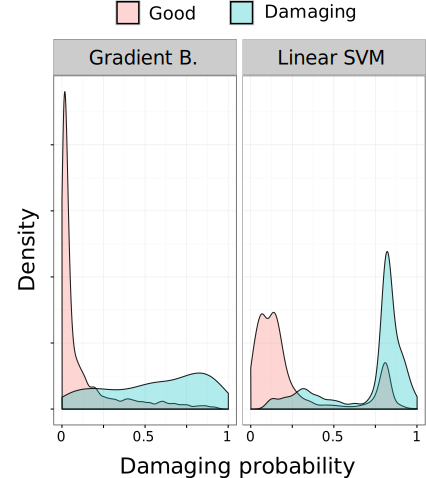
\includegraphics[width=.85\textwidth]{figures/natural_damaging_gb_vs_svc}
  \caption{No injected features}
  \label{fig:natural_damaging_gb_bs_svc}
\end{subfigure}~~
\begin{subfigure}[t]{.33\textwidth}
  \centering
  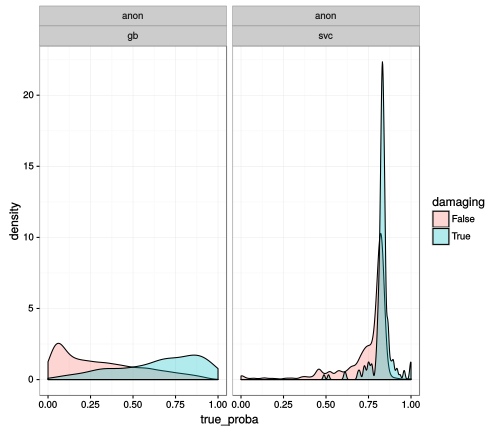
\includegraphics[width=.85\textwidth]{figures/anon_damaging_gb_vs_svc}
  \caption{Everyone is anonymous}
  \label{fig:anon_damaging_gb_bs_svc}
\end{subfigure}~~
\begin{subfigure}[t]{.33\textwidth}
  \centering
  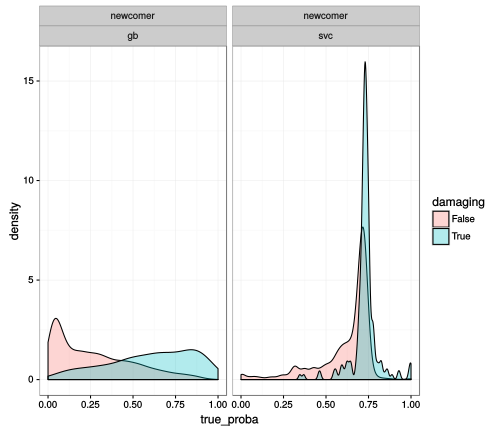
\includegraphics[width=.85\textwidth]{figures/newcomer_damaging_gb_vs_svc}
  \caption{Everyone is newly registered}
  \label{fig:newcomer_damaging_gb_bs_svc}
\end{subfigure}
\caption{The distributions of the probability of a single edit being scored as ``damaging'' based on injected features for the target user-class is presented.  Note that when injecting user-class features (anon, newcomer), all other features are held constant.}
\label{fig:prediction_error_for_anons_and_newcomers}
\end{figure*}

Shortly after we deployed ORES, we received reports that ORES's damage detection models were overly biased against anonymous editors.  At the time, we were using Linear SVM\footnote{\url{http://scikit-learn.org/stable/modules/generated/sklearn.svm.LinearSVC.html}} estimators to build classifiers, and we were considering making the transition towards ensemble strategies like GradientBoosting and RandomForest estimators.\footnote{\url{http://scikit-learn.org/stable/modules/ensemble.html}}  We took the opportunity to look for bias in the error of estimation between anonymous editors and newly registered editors.  By using our feature injection/interrogation strategy (described in Section~\ref{sec:innovations_in_openness}), we could ask our current prediction models how they would change their predictions if the exact same edit were made by a different editor.

Figure~\ref{fig:prediction_error_for_anons_and_newcomers} shows the probability density of the likelihood of ``damaging'' given three different passes over the exact same test set, using two of our modeling strategies.  Figure~\ref{fig:natural_damaging_gb_bs_svc} shows that, when we leave the features to their natural values, it appears that both models are able to differentiate effectively between damaging edits (high-damaging probability) and non-damaging edits (low-damaging probability) with the odd exception of a large amount of non-damaging edits with a relatively high-damaging probability around 0.8 in the case of the Linear SVM model.  Figures~\ref{fig:anon_damaging_gb_bs_svc} and \ref{fig:newcomer_damaging_gb_bs_svc} show a stark difference.  For the scores that go into these plots, characteristics of anonymous editors and newly registered editors were injected for all of the test edits.  We can see that the GradientBoosting model can still differentiate damage from non-damage while the Linear SVM model flags nearly all edits as damage in both case.

Through the reporting of this issue and our subsequent analysis, we were able to identify the issue and show that an improvement to our modeling strategy mitigates the problem.  Without such a tight feedback loop, we most likely would not have noticed how poorly ORES's damage detection models were performing in practice.  Worse, it might have caused vandal fighters to be increasingly (and inappropriately) skeptical of contributions by anonymous editors and newly registered editors---two groups of contributors that are already met with unnecessary hostility\footnote{\url{http://enwp.org/:en:Wikipedia:IPs_are_human_too}}\cite{halfaker2013rise}.


\section{Conclusion and future work}
\label{sec:conclusions_and_future_work}
Designing for empowerment leads us in new directions.  Rather than running an experiment on an ``intervention'' (e.g. \cite{halfaker2014snuggle}, we're reducing barriers and encouraging a ``conversation'' that has stalled to continue.  We see this as a ``hearing to speech'' ala Nell Morten\cite{morton1985journey} in contrast to ``speaking to be heard''.  By building the exact technology or process we think is right, we would be ``speaking to be heard'' and forcing our own views into the technological conversation about how quality is enacted in Wikipedia.  However, by stepping back and asking, ``What is preventing others from getting involved in this conversation?'' and lowering those barriers, we run the risk that the conversation will not go in the directions that we value.  It is a conscious choice we make to attempt to empower others rather than to assert ourselves, but we do not make this choice purely out of altruism.  It is simply impractical for one individual or small group to drive a conversation in Wikipedia in a productive direction.  Halfaker et al.'s Snuggle intervention\cite{halfaker2014snuggle} tried that strategy with limited success in past work.  We think it's time to hear to speech and see what others would like to contribute from their own standpoints.

When considering our design rationale, ORES is not quite a successor system.  It doesn't directly enact an alternative vision of how quality control should function in Wikipedia  It is a system for making the construction of successor technologies easier.  By solving for efficiency and letting others design for process, new, expanded standpoints can more easily be expressed.  Under another view, ORES is maybe a successor in that it enacts an alternative view of how algorithms should be made available to the populations they govern.  By keeping algorithms integrated into specific tools and keeping the operational details of the algorithm hidden, past developers enacted values of control and focused use of their creations.  By opening ORES as an algorithmic system, encouraging experimentation, and providing tools for interrogation of the algorithms themselves, we enact a set of values that embrace experimentation and the progress of mediation.

Still we do intend to help Wikipedia's social process form in ways that align with our values---the more complete balance of efficient quality control and newcomer support.  We want to see Wikipedia work better---and by ``better'' we mean that more people who want to contribute will feel welcome to do so and will find their place in Wikipedia.  However, in this paper we provide no direct evaluation of newcomer retention nor do we look for evidence of improved newcomer socialization.  Instead, we're targeting the early precursors of social change: reflection on the current processes and the role of algorithms in quality control.  We believe that the case studies that we describe both show that this reflection is taking place and that the wide proliferation of tools that provide surprising alternative uses of ORES suggest that  Wikipedians feel a renewed power over the their quality control processes.  Even if we are wrong about the direction of change that Wikipedia needs for quality control and newcomer socialization, we're inspired by much of the concern that has surfaced for looking into biases in ORES' prediction models (e.g. anons and the Italian ``ha'' from Section~\ref{sec:case_studies}) and the novel tools that volunteers are developing to support new editors (e.g. Ross's article quality recommender system from Section~\ref{sec:innovations_in_openness}).

\subsection{Future work}
One of the clear lines of future work that observing ORES in the world drives us toward is improved crowd-based auditing tools.  As our case studies suggest, auditing of ORES' predictions and mistakes has become a very popular activity.  Despite the difficulty for a user of finding a deep wiki page and using templates to flag false positives, Wikipedians have managed to organize several similar processes for flagging false positives and calling them to our attention.  In order to better facilitate this process, future system builders should implement structured means to refute, support, discuss, and critique the predictions of machine models.  With a structure way to report false positives and other real-human judgments, we can make it easy for tools that use ORES to also allow for reporting mistakes.  We can also make it easier to query a database of ORES mistakes in order to build the kind of thematic analyses that Italian Wikipedians showed us.  By supporting such an activity, we are working to transfer more power from ourselves and to our users.  Should one of our models develop a nasty bias, our users will be more empowered to coordinate with each other, show that the bias exists and where it causes problems, and eventually either get the model's predictions turned off or even shut down ORES.

We look forward to what those who work in the space of critical algorithm studies will do with ORES.  As of writing, most of the studies and critiques of \emph{subjective algorithms}\cite{tufekci2015algorithms} focus on large for-profit organizations like Google and Facebook---organizations that can't afford to open up their proprietary algorithms due to competition.  Wikipedia is one of the largest and most important information resources in the world.  The algorithms that ORES makes available are part of the decision process for allowing some people to contribute and preventing other.  This is a context where \emph{algorithms matter to humanity} and we are openly experimenting with the kind of transparent and open processes that the \emph{fairness and transparency} researchers are advocating.  Yet we have new problems and new opportunities.  There is a large body of work exploring how biases manifest and how unfairness can play out in algorithmically mediated social contexts.  ORES would be an excellent place to expand the literature within a real and important field site.

Finally, we also see potential in allowing Wikipedians, the denizens of Wikipedia, to freely train, test, and use their own prediction models.  Currently, ORES is only suited to deploy models that are developed by someone with a strong modeling and programming background.  However that doesn't need to be the case.  We have been experimenting with demonstrating ORES model building processes using Jupyter Notebooks\footnote{\url{http://jupyter.org}}\footnote{e.g. \url{ https://github.com/wiki-ai/editquality/blob/master/ipython/reverted_detection_demo.ipynb}} and have found that beginning programmers can understand the work involved.  This is still not the holy grail of crowd develop machine prediction---where all of the incidental complexities involved in programming are removed from the process of model development and evaluation.  Future work exploring strategies for allowing end-users to build models that are deployed by ORES would be a very interesting exploration of both the HCI issues involved and the changes the the technological conversations that such a margin-opening intervention might provide.


\section{Acknowledgements}
\label{sec:acknowledgements}
\input{sections/9_acknowledgements}

\section{Appendix}
See the supplementary material for the Appendix section.

% Bibliography
\bibliographystyle{ACM-Reference-Format}
\bibliography{refs}

\pagebreak
\appendix
\section{Appendix}
\label{sec:appendix}
\subsection{ORES system engineering}
\label{sec:ores_system_engineering}
In this section we describe how the system was designed in order to meet the needs of Wikipedian work practices and the tools that support them.

\subsubsection{Scaling \& robustness}


\subsubsection{Empirical access patterns}
\label{sec:appendix.empirical_access_patterns}
\begin{figure}[h]
\centering
\begin{subfigure}[t]{\columnwidth}
  \centering
  \includegraphics[width=.95\textwidth]{figures/ORES_request_activity_201804_week_vs_4hours}
  \caption{External requests per minute with a 4 hour block broken out to highlight a sudden burst of requests}
  \label{fig:ores_request_rate}
\end{subfigure}\\
\begin{subfigure}[t]{\columnwidth}
  \centering
  \includegraphics[width=.95\textwidth]{figures/ORES_precache_request_rate_201804}
  \caption{Precaching requests per minute}
  \label{fig:ores_precache_rate}
\end{subfigure}
\caption{Request rates to the ORES service for the week ending on April 13th, 2018}
\label{fig:ores_activity}
\end{figure}


The ORES service has been online since July 2015\cite{halfaker2015artificial}.  Since then, usage has steadily risen as we've developed and deployed new models and additional integrations are made by tool developers and researchers.  Currently, ORES supports 78 different models and 37 different language-specific wikis.

Generally, we see 50 to 125 requests per minute from external tools that are using ORES' predictions (excluding the MediaWiki extension that is more difficult to track).  Sometimes these external requests will burst up to 400-500 requests per second.  Figure~\ref{fig:ores_request_rate} shows the periodic and ``bursty'' nature of scoring requests received by the ORES service.  For example, every day at about 11:40 UTC, the request rate jumps---most likely a batch scoring job such as a bot.

Figure~\ref{fig:ores_precache_rate} shows the rate of precaching requests coming from our own systems.  This graph roughly reflects the rate of edits that are happening to all of the wikis that we support since we'll start a scoring job for nearly every edit as it happens.  Note that the number of precaching requests is about an order of magnitude higher than our known external score request rate.  This is expected, since Wikipedia editors and the tools they use will not request a score for every single revision.  This is a computational price we pay to attain a high cache hit rate and to ensure that our users get the quickest possible response for the scores that they \emph{do} need.

Taken together these strategies allow us to optimize the real-time quality control workflows and batch processing jobs of Wikipedians and their tools.  Without serious effort to make sure that ORES is practically fast and highly available to real-time use cases, ORES would become irrelevant to the target audience and thus irrelevant as a boundary-lowering intervention.  By engineering a system that conforms to the work-process needs of Wikipedians and their tools, we've built a systems intervention that has the potential gain wide adoption in Wikipedia's technical ecology.

\subsection{Explicit pipelines}
\label{sec:appendix.explicit_pipelines}
We have designed the process of training and deploying ORES prediction models to be repeatable and reviewable.  Consider the code shown in figure~\ref{fig:english_damaging_makefile} that represents a common pattern from our model-building Makefiles.

Essentially, this code helps someone determine where the labeled data comes from (manually labeled via the Wiki Labels system).  It makes it clear how features are extracted (using the \texttt{revscoring extract} utility and the \texttt{feature\_lists.enwiki.damaging} feature set).  Finally, this dataset of extracted features is used to cross-validate and train a model predicting the ``damaging'' label and a serialized version of that model is written to a file.  A user could clone this repository, install the set of requirements, and run \texttt{make enwiki\_models} and expect that all of the data-pipeline would be reproduced, and an equivalent model obtained.

By explicitly using public resources and releasing our utilities and Makefile source code under an open license (MIT), we have essentially implemented a turn-key process for replicating our model building and evaluation pipeline.  A developer can review this pipeline for issues knowing that they are not missing a step of the process because all steps are captured in the Makefile.  They can also build on the process (e.g. add new features) incrementally and restart the pipeline.  In our own experience, this explicit pipeline is extremely useful for identifying the origin of our own model building bugs and for making incremental improvements to ORES' models.

At the very base of our Makefile, a user can run \texttt{make models} to rebuild all of the models of a certain type.  We regularly perform this process ourselves to ensure that the Makefile is an accurate representation of the data flow pipeline.  Performing complete rebuild is essential when a breaking change is made to one of our libraries.  The resulting serialized models are saved to the source code repository so that a developer can review the history of any specific model and even experiment with generating scores using old model versions.

\begin{figure}[h]
        \makebox{\hrulefill}{
        \small
        \begin{verbatim}
datasets/enwiki.human_labeled_revisions.20k_2015.json:
    ./utility fetch_labels \
        https://labels.wmflabs.org/campaigns/enwiki/4/ > $@

datasets/enwiki.labeled_revisions.w_cache.20k_2015.json: \
        datasets/enwiki.labeled_revisions.20k_2015.json
    cat $< | \
        revscoring extract \
            editquality.feature_lists.enwiki.damaging \
            --host https://en.wikipedia.org \
            --extractor $(max_extractors) \
            --verbose > $@

models/enwiki.damaging.gradient_boosting.model: \
        datasets/enwiki.labeled_revisions.w_cache.20k_2015.json
    cat $^ | \
    revscoring cv_train \
        revscoring.scoring.models.GradientBoosting \
        editquality.feature_lists.enwiki.damaging \
        damaging \
        --version=$(damaging_major_minor).0 \
        -p 'learning_rate=0.01' \
        -p 'max_depth=7' \
        -p 'max_features="log2"' \
        -p 'n_estimators=700' \
        --label-weight $(damaging_weight) \
        --pop-rate "true=0.034163555464634586" \
        --pop-rate "false=0.9658364445353654" \
        --center --scale > $@
        \end{verbatim}
        \hrule
        \normalsize}
        \caption{Makefile rules for the English damage detection model from \url{https://github.com/wiki-ai/editquality}}
        \label{fig:english_damaging_makefile}
\end{figure}


\end{document}
